\documentclass[9pt,twoside,lineno]{pnas-new}
% Use the lineno option to display guide line numbers if required.

\templatetype{pnassupportinginfo}

\begin{document}


\title{Accelerated Inference for Partially Observed Stochastic Processes with Automatic Differentiation}
\author{Kevin Tan, Giles Hooker, Edward L. Ionides}
\correspondingauthor{Corresponding Author name.\\E-mail: kevtan@wharton.upenn.edu}


\maketitle


%% Comment out or remove this line before generating final copy for submission; this will also remove the warning re: "Consecutive odd pages found".
%\instructionspage  


%% Adds the main heading for the SI text. Comment out this line if you do not have any supporting information text.
\SItext


\subsection*{Subhead}


\begin{defn}[Targeting]
    \label{defn:targeting}
    A random vector $(X, w)$ drawn from a distribution $g$ \textbf{targets} the distribution $\pi$ if for any measurable and bounded functional $h$, $E_g\{h(X) \cdot w\}=E_\pi\{h(X)\}$ 
    A set of particles $(X^J_j, w^J_j), j=1,2, \ldots,J$, \textbf{targets} $\pi$ if for any measurable and bounded functional $h$
    ${\sum_{j=1}^J h(X^J_j) w^J_j}/{\sum_{j=1}^J w^J_j} \stackrel{a.s.}{\to} E_\pi(h(X))$ as $J\to\infty$
\end{defn}

\begin{lem}[Change of Particle Measure]
    \label{lem:change-measure-proper-weights}
    Assume $\{(\tilde X_j^J,U_j^J)\}_{j=1}^J$ targets $f_X$, and that $\{(Y_j^J,V_j^J)\}_{j=1}^J$ is a multinomial sample drawn from $\{(\tilde X_j^J,U_j^J)\}$ where $(\tilde X_j^J,U_j^J)$ is drawn w.p. $\pi^J_j$. Write, where $a$ is the ancestor function,
    $(Y_j^J,V_j^J) = \big(\tilde X^J_{a(j)},U^J_{a(j)}/\pi^J_{a(j)}\big)
    $. If the importance sampling weights $U_j/\pi_j$ are bounded, then $\{(Y^J_j,V^J_j)\}_{j=1}^J$ targets $f_X$.
\end{lem}
\begin{lem}[Particle Marginals]
    \label{lem:marginal-proper-weights}
    Suppose that $\{(\tilde X_j^J,U_j^J)\}_{j=1}^J$ targets $f_X$. Also suppose that $\tilde Z_j^J \sim f_{Z|X}(\cdot | \tilde X_j^J)$, where $f_{Z|X}$ is a conditional probability density function corresponding to a joint density $f_{X,Z}$ with marginal densities $f_X$ and $f_Z$. Then, if the $U_j^J$ are bounded, $\{(\tilde Z_j^J,U_j^J)\}_{j=1}^J$ targets $f_Z$.
\end{lem}
\begin{lem}[Particle Posteriors]
    \label{lem:posterior-proper-weights}
    Suppose that $\{(X_j^J,u_j^J)\}_{j=1}^J$ targets $f_X$, and write $(X^{\prime J}_j,u^{\prime J}_j) = \big(X_j^J,u_j^J \cdot f_{Z|X}(z^*|X_j^J)\big)$. Then, if $u_j^J \cdot f_{Z|X}(z^*|X_j^J)\big)$ and $u_j^J \cdot f_{Z|X}(z^*|X_j^J)\big) / f_Z(z^*)$ are bounded, $\{(X^{\prime J}_j,u^{\prime J}_j)\}_{j=1}^J$ targets $f_{X|Z}(\cdot | z^*)$.
\end{lem}
    
Whereas if we use the after-resampling conditional likelihoods $\hat\lik(\theta) = \prod_{n=1}^N L_n^{A,\theta,\alpha}$, the numerator of $L_n^{B,\theta,\alpha}$ is
\begin{equation}
    \sum_{j=1}^J g_{n,j}^\theta w_{n, j}^{P, \theta} = L^\phi_n \sum_{j=1}^J \left[ \frac{g^\theta_{n,j}}{g^\phi_{n,j}} w^{P,\theta}_{n,j}\right] \frac{g^\phi_{n,j}}{L_n^\phi}
\end{equation}
Using Lemma \ref{lem:change-measure-proper-weights}, we resample the corrected weights $w^{P,\theta}_{n,j}{g^\theta_{n,j}}/{g^\phi_{n,j}} $ according to probabilities ${g^\phi_{n,j}}/{L_n^\phi}$ to see this is properly estimated by $L^\phi_n \sum_{j=1}^J w^{F,\theta}_{n,j},$
from which we obtain the estimate $L_n^{B,\theta,\alpha}$. The strong consistency then follows as the likelihood is the product of the conditional likelihoods.


\begin{thm}[Consistency of MOP-$1$ Gradient Estimate]
    The gradient estimate of MOP-$\alpha$ when $\alpha=1$, $\theta=\phi$ is strongly consistent for the score. $\nabla_\theta \hat\ell_J^1(\theta) \stackrel{a.s.}{\to} \nabla_\theta \ell(\theta)$ as $J \to \infty$.
    \label{thm:mop-grad-consistency}
\end{thm}
\begin{proof}
    Fix $\omega \in \Omega$, and set $\phi = \theta$, where $\theta$ is the point we wish to evaluate the gradient at. The sequence $(\nabla_\theta \hat\lik_J^1(\theta)(\omega))_{J \in \mathbb{N}}$ is uniformly bounded over all $J$, by Assumption \ref{assump:local-bounded-derivative}. We claim that the sequence is also uniformly equicontinuous. To see this, by Assumption \ref{assump:local-bounded-derivative}, the second derivative of $\hat\lik_J^1(\theta)(\omega)|_{\theta=\theta'}$ is also bounded by $H'$ for almost every $\omega\in \Omega$ and every $\theta'\in \Theta$. A set of functions with derivatives bounded by the same constant is uniformly Lipschitz, and therefore uniformly equicontinuous. So the sequence $(\nabla_\theta \hat\lik_J^1(\theta)( \omega))_{J \in \mathbb{N}}$ is uniformly equicontinuous for almost every $\omega \in \Omega$. 
    Explicitly, for almost every $\omega \in \Omega$ and every $\epsilon>0$, there exists some $\delta(\omega)>0$ such that for every $||\theta - \theta'||_{\infty}<\delta$ and every $J \in \mathbb{N}$ we have that
    $$||\nabla_\theta \hat\lik_J^1(\theta)(\omega)-\nabla_\theta \hat\lik_J^1(\theta')(\omega)||_\infty < \epsilon.$$

    Then, by Arzela-Ascoli, there exists a uniformly convergent subsequence. We claim that there is only one subsequential limit. We know that as the gradient estimate is bounded by Assumption \ref{assump:local-bounded-derivative}, we can treat the gradient estimate at $\theta$ as a bounded functional of the particles. So by Theorem \ref{thm:mop-targeting} the sequence $(\nabla_\theta \hat\lik_J^1(\theta, \omega))_{J \in \mathbb{N}}$ converges pointwise for $\theta=\phi$ and almost every $\omega \in \Omega$, and there is therefore only one subsequential limit. The sequence therefore converges uniformly to its limit $\lim_{J \to \infty} \nabla_\theta \hat\lik_J^1(\theta)(\omega).$ Therefore, with uniform convergence for the derivatives established, we can swap the limit and derivative and obtain, in conjunction with the strong consistency $\hat{\lik}_J^1(\theta, \omega) \stackrel{a.s.}{\to} \lik(\theta)$ in Theorem \ref{thm:mop-targeting}, that for almost every $\omega \in \Omega$, 
    $$\lim_{J \to \infty} \nabla_\theta \hat\lik_J^1(\theta)(\omega) = \nabla_\theta \lim_{J \to \infty} \hat\lik_J^1(\theta)(\omega) = \nabla_\theta \lik(\theta).$$
    The result then follows by the continuous mapping theorem. 
\end{proof}


\section*{Heading}
\subsection*{Subhead}
Type or paste text here. You may break this section up into subheads as needed (e.g., one section on ``Materials'' and one on ``Methods'').

\subsection*{Materials}
Add a materials subsection if you need to.

\subsection*{Methods}
Add a methods subsection if you need to.


%%% Each figure should be on its own page
\begin{figure}
\centering
\includegraphics[width=\textwidth]{example-image}
\caption{First figure}
\end{figure}

\begin{figure}
\centering
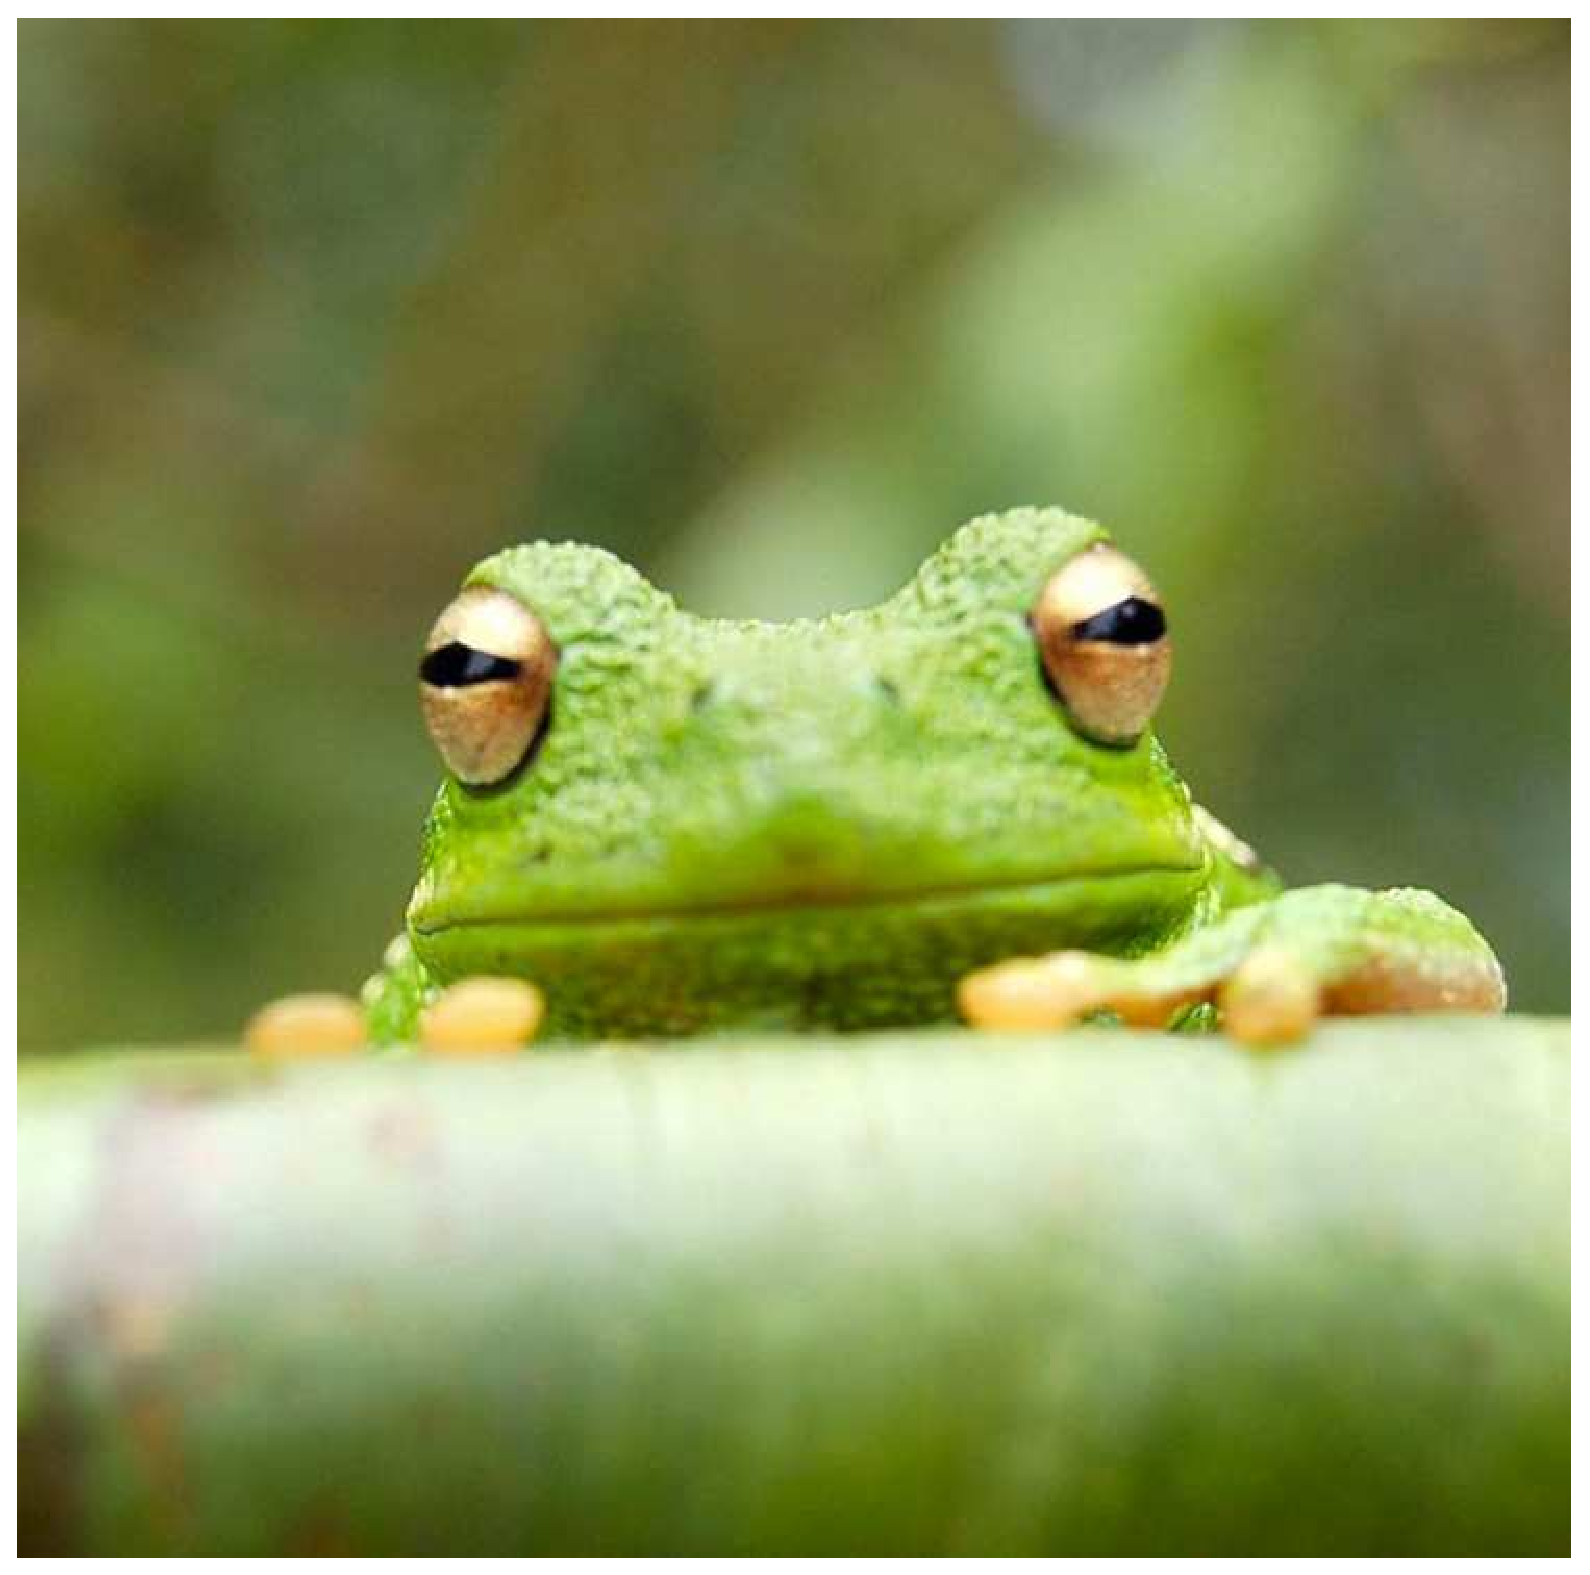
\includegraphics[width=\textwidth]{frog}
\caption{Second figure}
\end{figure}

\begin{table}\centering
\caption{This is a table}

\begin{tabular}{lrrr}
Species & CBS & CV & G3 \\
\midrule
1. Acetaldehyde & 0.0 & 0.0 & 0.0 \\
2. Vinyl alcohol & 9.1 & 9.6 & 13.5 \\
3. Hydroxyethylidene & 50.8 & 51.2 & 54.0\\
\bottomrule
\end{tabular}
\end{table}

%%% Add this line AFTER all your figures and tables
\FloatBarrier

\movie{Type legend for the movie here.}

\movie{Type legend for the other movie here. Adding longer text to show what happens, to decide on alignment and/or indentations.}

\movie{A third movie, just for kicks.}

\dataset{dataset_one.txt}{Type or paste legend here.}

\dataset{dataset_two.txt}{Type or paste legend here. Adding longer text to show what happens, to decide on alignment and/or indentations for multi-line or paragraph captions.}

\bibliography{pnas-sample}

\end{document}